%%%%%%%%%%%%%%%%%%%%%%%%%%%%%%%%%%%%%%%%%%%%%%%%%%%%%%%%%%%%%%%%%%% 
%                                                                 %
%                           CHAPTER 4                             %
%                                                                 %
%%%%%%%%%%%%%%%%%%%%%%%%%%%%%%%%%%%%%%%%%%%%%%%%%%%%%%%%%%%%%%%%%%% 
 
\chapter{Dramatic inner-core tropopause variability during the rapid intensification of {Hurricane Patricia} (2015)}
\resetfootnote %this command starts footnote numbering with 1 again.

%---------------------------------------------------------------------------------------%
\section{Introduction}
%---------------------------------------------------------------------------------------%

Hurricane Patricia became the strongest recorded hurricane in the Western Hemisphere after undergoing remarkably rapid intensification (RI) between 21 and 23 October 2015 (\citeauthor{Kimberlainetal2016} \citeyear{Kimberlainetal2016}; \citeauthor{Rogersetal2017} \citeyear{Rogersetal2017}).

Throughout this RI period, a NASA WB-57 aircraft flying in the stratosphere deployed 244 dropsondes as part of the Office of Naval Research Tropical Cyclone Intensity (TCI) Experiment \cite{DoyleTCI}.
These dropsondes revealed dramatic changes in upper-level static stability and cold-point tropopause structure throughout Patricia’s RI.

%---------------------------------------------------------------------------------------%
\section{Data and methods}
%---------------------------------------------------------------------------------------%
The High-Definition Sounding System (HDSS) provides a new capability to deploy and track up to 40 expendable digital dropsondes (XDDs) simultaneously.
This capability permits the rapid deployment of many dropsondes, providing cross sections of pressure, temperature, humidity, and wind velocity with unprecedented horizontal resolution.
\cite{Blacketal2017} report that XDDs are able to resolve atmospheric features in a manner comparable to RD-94 dropsondes \cite{HockFranklin1999}, operational rawinsondes, and aircraft spiral profiles.
The XDDs exhibited a warm bias of 18C and a dry bias of 5\% relative to RD-94 dropsondes.
XDD thermodynamic measurements, like those of other in situ sounding instruments, were noisy and unreliable when the sensors became wet.
An intensive quality control procedure \cite{BellTCI} removed unrealistic temperature and humidity observations that likely reflected sensor wetting, as well as relative humidity recorded at temperatures below -40\textdegree{}C, where humidity measurements were inaccurate because of slow sensor response time.
A more complete description of HDSS’s specifications and error characteristics can be found in \cite{Blacketal2017} and \cite{DoyleTCI}, and a comprehensive description of tihe quality control procedure in \cite{BellTCI}.

Flying near 18.5-km altitude aboard the NASA WB-57 aircraft, HDSS deployed dropsondes with horizontal spacing as small as 4 km in the inner core of TC Patricia.
This dataset builds upon that of the high-altitude dropsonde observations collected by the NASA Hurricane and Severe Storm Sentinel (HS3) investigation \cite{Braunetal2016}.
Although many dropsondes were deployed during each HS3 flight, the typical spacing of 50–200 km was not sufficient to resolve the inner core of a hurricane. In contrast, the average dropsonde spacing for the four complete transects that TCI conducted through the center of TC Patricia ranged from 4.4 to 8.0 km. 
These four flight legs, shown in Fig.~\ref{fig:patricia_ir}, will be used to analyze the upper-tropospheric and lower-stratospheric evolution of TC Patricia during its RI.

The infrared (IR) brightness temperature images plotted in Fig.~\ref{fig:patricia_ir} were parallax-corrected using Man
computer Interactive Data Access System (McIDAS-X; \citeauthor{Lazzaraetal1999} \citeyear{Lazzaraetal1999}), assuming a cloud-top height of 15 km.
For each transect, the parallax adjustment was determined at every dropsonde position and the IR image was shifted by the average of these adjustment factors.
This effectively shifted the IR image 9 km to the southeast on 21 October (when the satellite image came from GOES-13) and 13 km to the southwest on 22 and 23 October (when the satellite image came from GOES-15).
This parallax adjustment was performed only to show more realistic dropsonde deployment locations relative to the IR brightness temperatures in Fig.~\ref{fig:patricia_ir}; it did not impact any calculated field.

Each sounding in the quality-controlled TCI dropsonde dataset \citep{BellTCI} was interpolated to a 100-m vertical grid following \cite{MolinariVollaro2010}.
The static stability was analyzed using the squared Brunt–V{\"a}is{\"a}l{\"a} frequency:
   \begin{equation} \label{eq:n2dry}
   N^2 = \frac{g}{\theta}\frac{\Delta \theta}{\Delta z},
   \end{equation}
where $\Delta z$ is 200 m.
The vertical temperature gradient, $\Delta T/\Delta z$, also was computed across 200-m layers using centered finite differences.

The evolution of $\theta$ anomalies will be used to aid the diagnosis of static stability changes.
Although many previous papers have used the \cite{Jordan1958} or \cite{Dunion2011} mean soundings to compute temperature anomalies, neither of these soundings are representative of the environment in which Patricia was embedded.
For this reason, a mean state was defined using an average of 74 rawinsonde observations obtained from the University of Wyoming upper-air sounding archive \citep{Wyoming2016}.
These observations constituted all rawinsondes released from Manzanillo and Acapulco, Mexico, during October 2015. Each sounding was visually inspected for errors and three soundings from Manzanillo were removed from the average: 0000 UTC 6 October, 1200 UTC 11 October, and 1200 UTC 21 October.
These soundings exhibited unrealistically large upper-tropospheric temperature departures relative to the previous and subsequent soundings.
Their removal did not significantly alter the mean sounding: the maximum difference in the average temperatures computed with and without those soundings was 0.47\textdegree{}C. 
A total of 58 of the 74 rawinsondes reported data up to at least the 19-km level, facilitating the computation of $\theta$ anomalies well into the lower stratosphere.

For each cross section, the storm center location was determined using a wind center track produced by NOAA’s Hurricane Research Division (available online at \url{http://www.aoml.noaa.gov/hrd/Storm_pages/patricia2015/patricia.trak}).
The WB-57 dropsonde deployment location nearest this storm center estimate in space and time was used to define the center (radius = 0) for each cross section.
The distance between the nearest dropsonde and the storm track never exceeded 8.1 km (Table~\ref{table1}).
Storm-relative radial and tangential velocities were computed using the speed and direction of motion along this track.

%---------------------------------------------------------------------------------------%
%FIGURES AND TABLES
%---------------------------------------------------------------------------------------%

%Table 1%

\begin{table}
  \scriptsize
 \begin{center}
   \begin{tabular}{ c c c c }
   Time and Date & Storm center from HRD track & Location of nearest WB-57 dropsonde deployment & Separation distance\\
   \hline
   \hline
   1957:00 UTC 21 Oct & 13.056\textdegree{}N, 99.244\textdegree{}W & 12.983\textdegree{}N, 99.235\textdegree{}W & 8.1 km\\
   1823:15 UTC 22 Oct & 15.123\textdegree{}N, 104.149\textdegree{}W & 15.101\textdegree{}N, 104.142\textdegree{}W & 2.5 km\\
   1906:00 UTC 22 Oct & 15.238\textdegree{}N, 104.247\textdegree{}W & 15.204\textdegree{}N, 104.237\textdegree{}W & 3.9 km\\
   2001:30 UTC 23 Oct & 18.617\textdegree{}N, 105.199\textdegree{}W & 18.590\textdegree{}N, 105.207\textdegree{}W & 3.1 km\\
   \hline
   \end{tabular}
 \end{center}
 \caption{Storm center positions from NOAA’s Hurricane Research Division (HRD) zero wind center track for Hurricane Patricia, the nearest WB-57 dropsonde deployment location, and the distance (km) between the two points.}
 \label{table1}
\end{table}

%FIGURE 1%
\begin{figure*}[ht]
\centerline{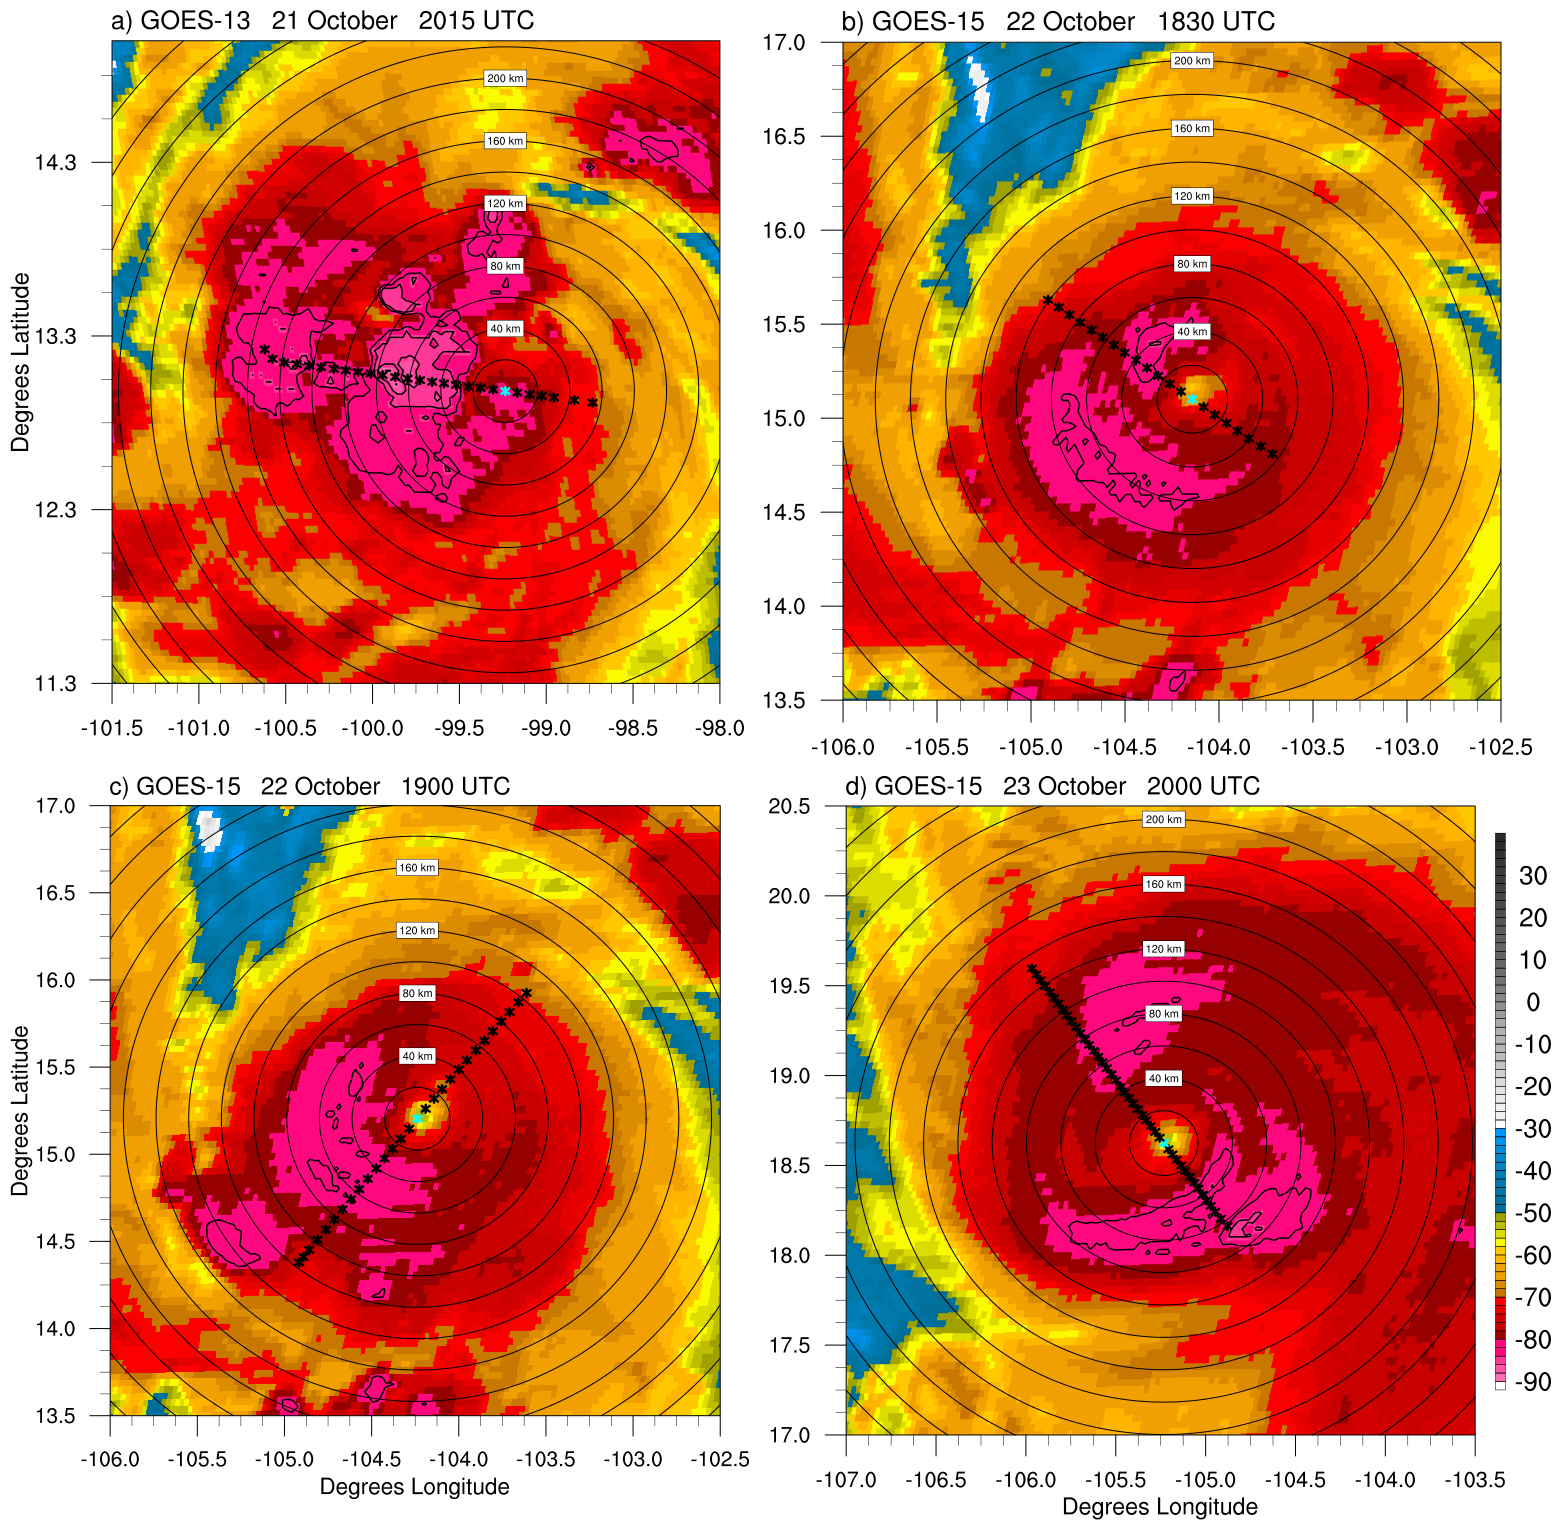
\includegraphics[width=39pc]{figures/fig01_patricia_ir.png}}
\caption{Infrared brightness temperature (\textdegree{}C) images of Tropical Storm Patricia at (a) 2015 UTC 21 Oct, and Hurricane Patricia at (b) 1830 UTC 22 Oct, (c) 1900 UTC 22 Oct, and (d) 2000 UTC 23 Oct 2015. Stars represent dropsonde deployment locations, with cyan stars marking the center location used for each cross section. Black contours delineate the coldest brightness temperatures, with a contour interval of 2\textdegree{}C starting at -82\textdegree{}C. The mean dropsonde spacing is (a) 7.9, (b) 7.8, (c) 8.0, and (d) 4.4 km for the four flight legs. Range rings are plotted every 20 km.}
\label{fig:patricia_ir}
\end{figure*}
